\documentclass[paper=a4,fontsize=11pt]{temp} % KOMA-article 
\usepackage{array}

\usepackage[%
  colorlinks=true,%
  urlcolor=blue%
]{hyperref}
\newcommand{\at}{\makeatletter @\makeatother}
\usepackage{color}
\definecolor{redCV}{RGB}{88,24,37}
\definecolor{blueCV}{RGB}{36,82,139}


\begin{document}
%\sepspace
\begin{minipage}{.21\linewidth}
  % 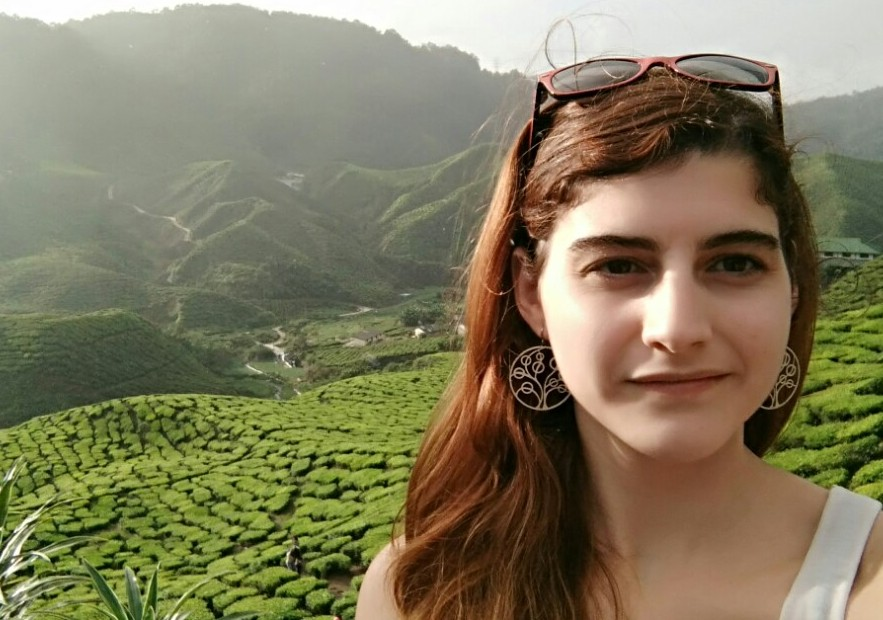
\includegraphics[width=1.4\textwidth]{ana2}
   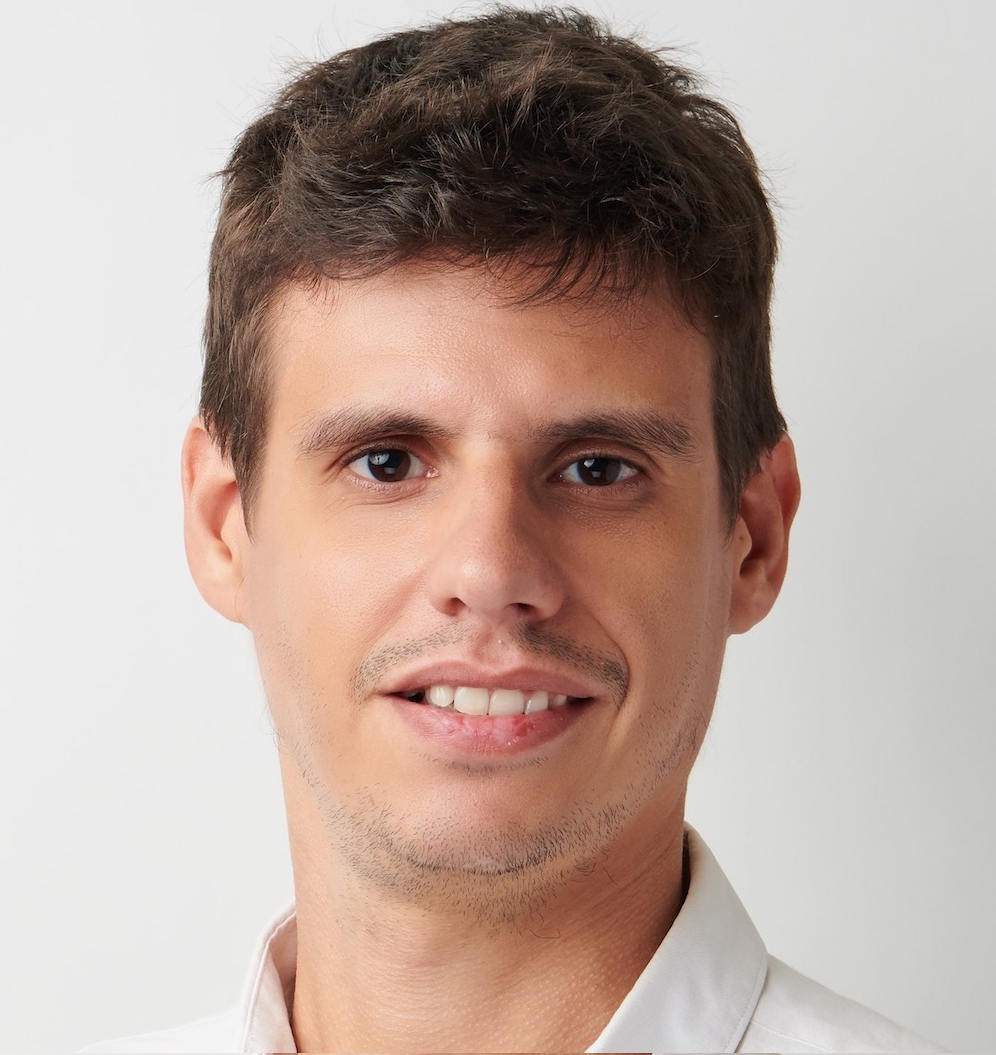
\includegraphics[width=1.05\textwidth]{PicQuim2019}
   \vspace{2pt}
\end{minipage}      
\begin{minipage}{0.705\linewidth}
   \MyName{Joaquim Bellmunt Montoya, Ph.D.}
   \sepspace
   \noindent
   
   \hfill    
   \begin{tabular}[width=\textwidth]{@{}cl@{}}
   \setlength{\tabcolsep}{12pt}
   \begin{tabular}{>{\centering\arraybackslash}p{.5\textwidth}} \centering \small \textit{Technological innovations that allows the interoperability between agents and the better context understanding.\\NLP, Knowledge Graph, Open Linked Data and Internet of Things.\vspace{2ex}} \end{tabular}
   & \setlength{\tabcolsep}{5pt} \begin{tabular}{@{}cl@{}}
    
\includegraphics[height=2ex]{IMG/icons/map5}  & Singapore\\
    
\includegraphics[height=2ex]{IMG/icons/profile} & Barcelona, Oct 15th 1987  \\%\begin{tabular}{@{}c@{}}
    
\includegraphics[height=2ex]{IMG/icons/mail9}%\vspace{-.1ex}\end{tabular}
    & \href{mailto:joaquim.bell@gmail.com}{\color{blueCV}{joaquim.bell@gmail.com}} \\
    
\includegraphics[height=2ex]{IMG/icons/telephone1} &(+65) 81193783 \\  
    
\includegraphics[height=2ex]{IMG/icons/social6}  &  quimbell\\    
    
\includegraphics[height=2ex]{IMG/icons/social22}  &  \href{https://es.linkedin.com/in/joaquimbellmunt
}{\color{blueCV}{joaquimbellmunt}}        
   \end{tabular}
 \end{tabular}
   %\hfill yourwebsite.com  
   %\hfill (+351)93123123123  
\end{minipage}
\vspace{-2ex}

\NewPart{Work experience}{}
\noindent

\workEntry{Accenture Pte.}{Feb 2018 - Present}{NLP \& Knowledge Graph SME}{I Joined Accenture after the Ph.D. defense to develop the Knowledge Graph Practice and provide to client the best cloud experience in the data management. Also involved in NLP projects to ensure the high standards quality and interoperability\color{blueCV}{Knowledge Graph, NLP, Semantic Web, Open Linked Data, Graph Analytics.}}{IMG/accenture.png}
Highligted Project:
$\bullet$ Changi Airport Chatbot
$\bullet$ Knowledge Graph Rapid Prototyping Asset
$\bullet$ Big Data Cloud Data Lake Architect 
\sepspace

\workEntry{Pixium Digital Pte ltd.}{collaboration upon request}{Artificial Intelligence Consultant}{Pixium Digital was founded in 2015 by Digital market experts and experienced developers with the goal of providing everyone with a customised digital solution: \color{blueCV}{Mobile Development, Data Science, IoT, ML and Knowledge Aggregation.}}{IMG/pixium.png}
\sepspace

\workEntry{Image and Pervasive Access Lab (CNRS UMI)}{Jul 2014 - Nov 2017}{Research Assistant}{Ph.D. Student attachment.
focusing on Semantic Reasoning, Data Mining, Human Condition Computation and Context-Aware Service Delivery in Ambient Assisted Living deployments for Ageing in Place. \textbf{Ambient Assisted Living Framework presentation:} \href{http://bit.ly/2lkgiqh}{\color{blueCV}{UBISmart v4.0}}} {IMG/ipal.eps}
\sepspace

\hspace{3mm}
\begin{minipage}{0.04\linewidth}
        \hspace{\linewidth}
		\end{minipage}
   \begin{minipage}{0.86\linewidth}
   	\hspace{2ex}
	 \textbf{\color{subheadings}{Project Management}}  
   \begin{itemize}
  \item \textbf{City4Age and Pulse (HORIZON 2020)} System Architect and Technical Project Manager in 2 Pilot sites (Singapore and Montpellier) in a European project focusing on the use of IoT technologies to help frail elderly to live with independence and safety. 
%   The technologies used include: Raspberry Pi, X10 and Z-Wave sensors and beacons; Cloud computing (AWS EC2and DigitalOcean), RESTFul and OpenData API aggregation; MQTT client and broker; code development on NodeJs, Python and Android; etc.  %In charge of planning the technical implementation; hardware provisioning, Raspberry Pi, X10 and Z-Wave sensors and beacons; code development, web server on AWS and android applications; system deployment and integration in real deployments; and maintenance and improvements in ongoing deployments.
   %\item\textbf{2017 Call for Projects HORIZON 2020}: Contribution in the technical work packages in a European project proposal for Aging and Wellbeing. The project focuses on the inclusion of new IoT technologies to enhance the quality of life of active aging (Mobile App, Connected Objects, and Open Data).
   %\item \textbf{Ambient Assisted Living platform video presentation:} \href{http://bit.ly/2lkgiqh}{UBISmart v4.0}
   \end{itemize}
\end{minipage}
%\workEntrySmall{Nanyang Techonological University}{Fall 2016}{Teaching Assistant}{Teacher at the Algorithms CE2001 module lab.}{IMG/NTUE}

\sepspace

\sepspace

\workEntrySmall{KPMG}{Nov 2013 - Apr 2014}{IT Auditor}{Systems Auditor for annual audits in several multinational companies.}{IMG/kpmg}

\sepspace

\workEntry{LIRMM}{Mar 2013 - Sep 2013}{Research Intern}{%Intern at the Laboratoire d'Informatique, Robotique et Micro-Éléctronique de Montpellier. 
Master Thesis Internship in Medical Robotics.} {IMG/lirmm}

\sepspace

\workEntrySmall{Dept. of Signal Theory and Communications}{Feb 2011 - Jan 2012}{Fellow Intern}{%Intern at UPC. In charge of 
Part of my responsibilities were the computer maintenance and support for all department staff.}{IMG/upc}


%\sepspace

%\workEntrySmall{Centre Municipal de Vela Barcelona}{2008-2011}{Sailing Instructor}{Summer sailing courses for kids of all ages and adults.}{IMG/cmv}


\NewPart{Education}{}
\noindent


\EducationEntry{Ph.D. in Computer Science}%at IPAL
{Jul 2014 - Nov 2017}{Institut Mines-Télécom, University of Montpelier (CNRS UMI), France}{3 years Ph.D. Program in Computer Science.} {IMG/imt}%{Institut Mines-télécom, French Ph.D. in Singapore at IPAL (CNRS UMI)} {IMG/imt}

\sepspace


% \EducationEntry{ICT for Health Specialisation}{Sep 2012 - Sep 2013}{Institut Mines-Télécom, Université Montpellier, École des Mines d'Alès, Montpellier, France}{Master Degree with Specialty in Information and Technology in the Health field.} {IMG/imt}

% \sepspace


\EducationEntry{MSc. in Telecommunications Engineering}{Feb 2012 - Sep 2013}{ENS Telecom Bretagne, Brest, France}{Double Master Degree program with TelecomBCN.} {IMG/brest}

\sepspace


\EducationEntry{BSc and MSc. in Telecommunications Engineering}{Sep 2005 - Jan 2012}{TelecomBCN (ETSETB, UPC Barcelona Tech), Spain}{Modules in Probability \& Statistics, Data \& Signal Processing, Telematics, Communications, \textit{etc}.}{IMG/logo_telecom_S}

\pagebreak
%\sepspace

% \NewPart{Skills \& Interests}{}
% \hspace{3mm}
% \begin{minipage}[t]{0.33\textwidth} 

% \begin{tabular}[t]{ l l }
% \vspace{0.75ex}
% \flag{IMG/flag/es}  & Native Speaker \\
% \vspace{0.75ex}
% \flag{IMG/flag/cat} & Native Speaker \\
% \vspace{0.75ex}
% \flag{IMG/flag/fr}  & Bilingual \\
% \vspace{0.75ex}
% \flag{IMG/flag/gb}  & Full Competence
% \end{tabular}

% \sepspace

% \end{minipage}
%
\NewPart{Skills}{}
\noindent
\begin{minipage}[t]{\textwidth} 

\begin{tabular}[t]{l l}
\softwareb{IMG/icons/language}  	 &\small \begin{tabular}[t]{@{}l@{}} 
     \flag{IMG/flag/es} Native Speaker; \flag{IMG/flag/cat} Native Speaker; \flag{IMG/flag/fr}  Bilingual; \flag{IMG/flag/gb}  Full Competence 
\end{tabular} \vspace{.7ex}
\\
\softwareb{IMG/soft/computer}  	 &\small \begin{tabular}[t]{@{}l@{}} 
     $\bullet$ \textbf{\textcolor{blueCV}{Cloud Technology: }} GCP; AWS; Watson; Azure, Datastax.\\
     $\bullet$ \textbf{\textcolor{blueCV}{ML/DL: }} TensorFlow; Keras; NLTK; TensorBoard; PyTorch.\\
     $\bullet$ \textbf{\textcolor{blueCV}{KG/Semantic Web: }}   RDF/OWL; N3; LOD; Python and NodeJs wrappers; Property Graph; TinkerPop; Cypher.\\
	 $\bullet$ \textbf{\textcolor{blueCV}{Data Management: }} RDF Triples; MySQL; Postgresql;MySQL; MongoDB.\\
	 $\bullet$ \textbf{\textcolor{blueCV}{Coding: }} JavaScript; Java; Python; N3; Bash; R; Git.\\
\end{tabular} \vspace{.7ex}
\\


\softwareb{IMG/foot}  &\small\setlength\extrarowheight{-1ex}\begin{tabular}[t]{@{}p{.8\linewidth}@{}}
Sportive, specially Football, and Barça fan. Cinema, traveling, driving.
\end{tabular} \\
\end{tabular}
\end{minipage}

\setlength\extrarowheight{-1ex}
\vspace{1ex}
\begin{tabular}{l l}
%
\softwareb{IMG/people}  &\small  \begin{tabular}[t]{@{}p{.85\linewidth}@{}}
$\bullet$ Founder and Manager of two football teams in Singapore regrouping European people.\\[1ex]

$\bullet$ Board member of \href{www.telecogresca.com}{\color{blueCV}{Telecogresca}} in 2011 and 2012. Telecogresca is a student association, which organizes a music festival hosting every year more than 10.000 people. Former Vice-President of the sports student association at TelecomBCN, CET, which organizes every semester different sportive competitions, such as Football, Basketball or Volleyball.
\end{tabular} 
\end{tabular}

%\sepspace

\NewPart{PUBLICATIONS}{} %PROFESSIONAL ACTIVITIES
\hspace{3mm}
\begin{minipage}{0.04\linewidth}
        \hspace{\linewidth}
		\end{minipage}%  
   \begin{minipage}{0.88\linewidth}
   %\noindent\hangindent=2em\hangafter=1 
\iffalse   
   \textbf{\color{subheadings}{Projects}}
   
$\bullet$ \textbf{City4Age (HORIZON 2020)} System Architect and Technical Project Manager in 2 Pilot sites in 18 months European project focusing on the use of technologies to help frail aging to live with independence and safety. In charge of communicating with end-users to understand the needs and adjust objectives. Also in planning the technical implementation; hardware provisioning; code development; system deployment and integration; and maintenance and improvements.\vspace{1ex}

$\bullet$ \textbf{2017 Call for Projects HORIZON 2020}: Contribution in the technical work packages in a European project proposal for Aging and Wellbeing. The project focus on the inclusion of new technologies to enhance the quality of life of active aging (Mobile App, Connected Objects, and Open Data).
\vspace{1.5ex}
   
   \textbf{\color{subheadings}{Publications}}
\fi
\begin{footnotesize}

$\bullet$ Kodys, M., Oliver, P., \textbf{\textcolor{blueCV}{Bellmunt, J.}}, Aloulou, H., Kaddachi, F. \& Mokhtari, M. Smart Mobility in Urban Assisted Living Environments. In \textit{Information Integration and Web-based Applications \& Services}, 2017. \textit{Accepted}

$\bullet$ Kodys, M., \textbf{\textcolor{blueCV}{Bellmunt, J.}}, Aloulou, H. \& Mokhtari, M. Oh, wait, reasoning was wrong! Let's replay. In \textit{Semantic Web Technologies for the Internet of Things}, 2017. \textit{Accepted}

$\bullet$ \textbf{\textcolor{blueCV}{Bellmunt, J.}}, Mokhtari, M., Abdulrazak \& B., Aloulou. Validation of an Ubiquitous Computational Frailty Model Towards an Adaptable Ambient Assisted Living Framework. In \textit{Proceedings of the ACM on Interactive, Mobile, Wearable and Ubiquitous Technologies \& UbiComp. 3rd Issue Nov}. ACM, 2017. \textit{Under Review}

%$\bullet$ \textbf{\textcolor{blueCV}{Bellmunt, J.}}, Mokhtari, M., Abdulrazak, B., Aloulou, H. \& Kodys, M. UbiFrailty: Ubiquitous Computational Frailty Model Towards an Adaptable Service Provisioning. In \textit{Wireless Communications and Mobile Computing, Internet of Things and Smart Environments Supporting Healthy Ageing Services (Special Issue)}. Hindawi, 2017. \textit{Under Review}
 
$\bullet$ Aloulou H., Endelin R., Mokhtari M., Abdulrazak B., Kaddachi F., \textbf{\textcolor{blueCV}{Bellmunt, J.}} Activity Recognition Enhancement Based on Ground-Truth: Introducing a New Method Including Accuracy and Granularity Metrics. In \textit{ICOST}. Springer, 2017.

%$\bullet$ \textbf{\textcolor{blueCV}{Bellmunt, J.}}, Aloulou, H., Montalva J.B., Clavier, F., Rios, S. \& Mokhtari, M. Active and Healthy Aging City Services for MCI and Frailty Prevention: Test Beds Approach. In \textit{Software, Telecommunications and Computer Networks (SoftCOM 2017)}. 2017. \textit{Accepted}
  

$\bullet$ Sadek, I., \textbf{\textcolor{blueCV}{Bellmunt, J.}}, Kodyš, M. \& Mokhtari, M. Novel Unobtrusive Approach for Sleep Monitoring Using Fiber Optics in an Ambient Assisted Living Platform. In \textit{ICOST}. Springer, 2017.

$\bullet$ Kadachi, F., Aloulou, H., Abdulrazak, B., \textbf{\textcolor{blueCV}{Bellmunt, J.}}, Endelin, R., Mokhtari, M. \& M.Fraisse, P. Technological Approach for Behavior Change Detection toward Better Adaptation of Services for Elderly People. In \textit{Health Informatics}. 2017.
 

$\bullet$ \textbf{\textcolor{blueCV}{Bellmunt, J.}}, Mokhtari, M., Abdulrazak, B. \& Aloulou, H.  Agile Framework for Rapid Deployment in Ambient Assisted Living Environments. In \textit{Information Integration and Web-based Applications and Services}. ACM, 2016.


$\bullet$ Aloulou, H., Abdulrazak, B., Endelin, R., Kadachi, F. \& \textbf{\textcolor{blueCV}{Bellmunt, J.}}. Detecting Inconsistencies in Rule-Based Reasoning for Ambient Intelligence. In \textit{Engineering of Complex Computer Systems (ICECCS)}. IEEE, 2016.


$\bullet$ \textbf{\textcolor{blueCV}{Bellmunt, J.}}, Mokhtari, M., Abdulrazak, B., Aloulou, H. \& Kodys, M. Experimental Frailty Model Towards an Adaptable Service Delivery for Aging People. In \textit{Engineering of Complex Computer Systems (ICECCS)}.IEEE, 2016.

$\bullet$ Aloulou, H., Abdulrazak, B., Endelin, R., Bentes, J., Tiberghien, T. \& \textbf{\textcolor{blueCV}{Bellmunt, J.}}. Simplifying Installation and Maintenance of Ambient Intelligent Solutions Toward Large Scale Deployment. In \textit{ICOST}. Springer 2015.

$\bullet$ \textbf{\textcolor{blueCV}{Bellmunt, J.}}, Tiberghien, T., Mokhtari, M., Aloulou, H. \& Endelin, R. Technical Challenges Towards an AAL Large Scale Deployment. In \textit{ICOST}. Springer, 2015.

\end{footnotesize}

 \end{minipage} 


%\sepspace

%\NewPart{Honors \& Awards}{}
\NewPart{Courses \& Awards}{}\begin{minipage}{0.065\linewidth}
	\hspace{\linewidth}
\end{minipage}%  
\begin{minipage}{0.88\linewidth}
\vspace{-1ex}
\textbf{\color{subheadings}{Courses}}\\
\begin{footnotesize}
$\bullet$ Google Cloud Platform Big Data and Machine Learning Fundamentals, 2017 (Coursera) \\
$\bullet$ Semantic Web Summer School, 2015 (SWSS)\\
$\bullet$ Machine Learning,2014 (Coursera) \\
$\bullet$ OpenHPI, Semantic Web Technologies, 2013 (OpenHPI)\\
\end{footnotesize}
\vspace{1.5ex}
\textbf{\color{subheadings}{Awards}}
\vspace{1ex}

\AwardEntryLong{IoT Hackathon}{Apr 2015}{I²R/A*STAR - ETPL - SIAA}{First Runner Up  at IoT Hackathon organized by I²R/A*STAR - ETPL - SIAA}{IMG/A-STAR}


\end{minipage}
% \hspace{3mm}
% \begin{minipage}[t]{0.88\textwidth}
% \AwardEntry{IoT Hackathon}{Apr 2015}{First Runner Up  at IoT Hackaton organized by I²R/A*STAR - ETPL - SIAA} {IMG/A-STAR}
% \end{minipage}

% \hspace{0.02\textwidth}
% \begin{minipage}[t]{0.45\textwidth}
% \AwardEntry{Obra Social "La Caixa"}{Apr 2015}{Scholarship to cover additional conference and travel expenses during my PhD.} {IMG/lacaixa}
% \end{minipage}



% \NewPart{Referees}{}
% \hspace{3mm}
% \begin{minipage}[t]{0.45\textwidth}
% %\RefereeEntry{Prof. Mounir Mokhtari}{}{Ph.D. director \\ IPAL Director \\ Professor at Institut Mines-Télécom\\
% %\href{mounir.mokhtari@ipal.cnrs.fr}{mounir.mokhtari@ipal.cnrs.fr}} {pics/mounir}

% \RefereeEntryB{Prof. Mounir Mokhtari}{IPAL \& Institut Mines-Télécom}{Ph.D. Director \\ IPAL Director \\
% \href{mounir.mokhtari@ipal.cnrs.fr}{mounir.mokhtari@ipal.cnrs.fr}} {pics/blank}
% \end{minipage}
% %\hspace{0.02\textwidth}
% \begin{minipage}[t]{0.45\textwidth}
% %\RefereeEntry{Prof. Bessam Abdulzarak}{}{Ph.D. advisor\\ Professor at University of Sherbrooke\\ Invited Professor at LIRMM\\ \href{bessam.abdulrazak@usherbrooke.ca}{bessam.abdulrazak@usherbrooke.ca}} {pics/Bessam}

% % \RefereeEntryB{Prof. Bessam Abdulzarak}{University of Sherbrooke}{Ph.D. Advisor\\Invited Professor at LIRMM\\ \href{bessam.abdulrazak@usherbrooke.ca}{bessam.abdulrazak@usherbrooke.ca}} {pics/Bessam}
% \end{minipage}
%  \sepspace
 


%%% References
%%% ------------------------------------------------------------

\end{document}
